% !TeX root = ../main.tex

\appendix{A}{各數學公式}
\section{動量守恆證明}
\begin{figure*}[ht!]
    \centering
    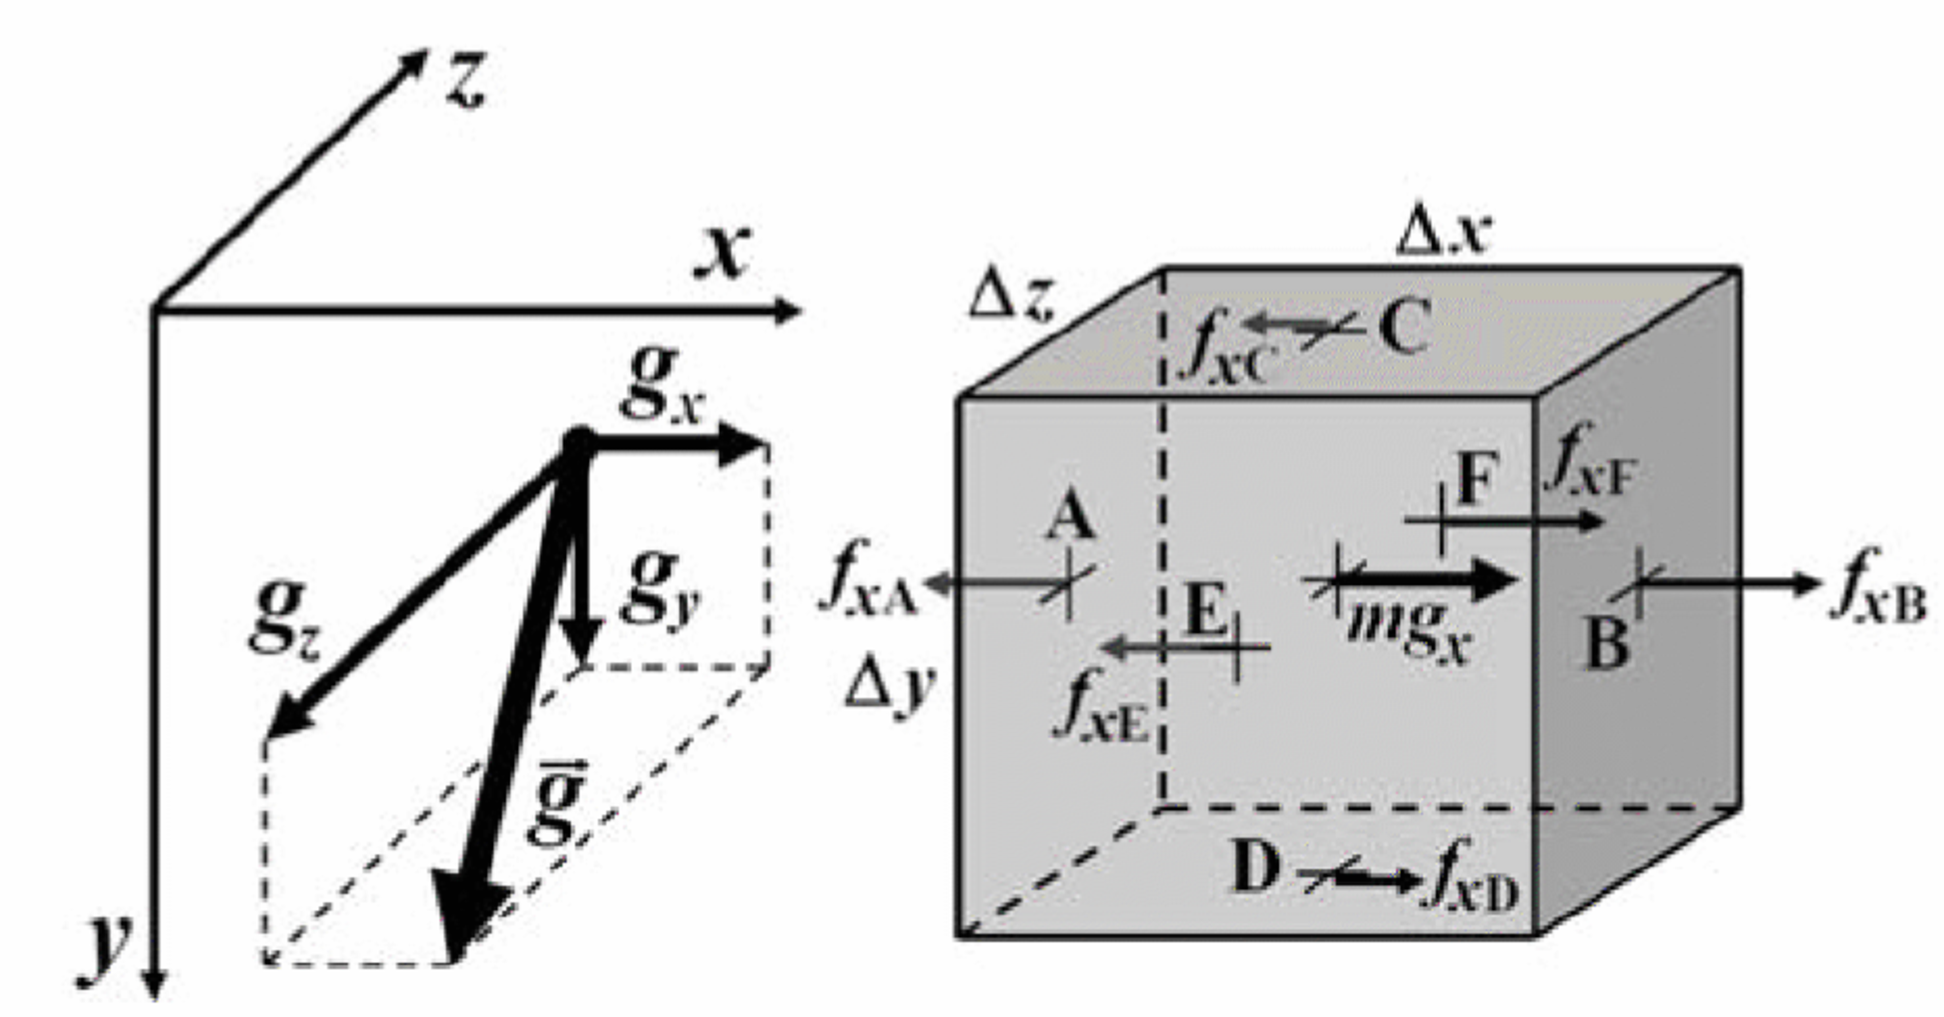
\includegraphics[width=4in]{momentum.pdf}
    \caption{ 拉格朗日體積示意圖,摘自\citet{Gerya2009}}
    \label{fig::Lagrangian Volume Momentum}
\end{figure*}
利用計算作用於一小拉格朗日體積上之淨力(net forces)可證明$\ref{eqn:momentum Lagrangian}$:

對x分量而言,
\begin{align}
f_x=f_{xA}+f_{xB}+f_{xC}+f_{xD}+f_{xE}+f_{xF}+mg_x \label{eqn:Ftotal0}
\end{align}
$f_{xA}- f_{xF}$ 為與應力相關之力,其來自於各邊界A-F上體積外部。 
$f_g=m_gx$ 為重力。

\begin{align}
f_{xA} = -\sigma_{xxA}\Delta y\Delta z\label{eqn:fxA}\\
f_{xB} = +\sigma_{xxB}\Delta y\Delta z\label{eqn:fxB}\\
f_{xC} = -\sigma_{xyC}\Delta x\Delta z\label{eqn:fxC}\\
f_{xD} = +\sigma_{xyD}\Delta x\Delta z\label{eqn:fxD}\\
f_{xE} = -\sigma_{xzE}\Delta x\Delta y\label{eqn:fxE}\\
f_{xF} = +\sigma_{xzF}\Delta x\Delta y\label{eqn:fxF}
\end{align}
將($\ref{eqn:fxA}$)-($\ref{eqn:fxF}$)帶入($\ref{eqn:Ftotal0}$)中得到:
\begin{align}
(\sigma_{xxB}-\sigma_{xxA})\Delta y\Delta z+(\sigma_{xyD}-\sigma_{xyC})\Delta x\Delta z+(\sigma_{xzF}-\sigma_{xzE})\Delta x\Delta y+mg_x = ma_x 
\end{align}
透過拉格朗日體積對左右兩式進行正交化:
\begin{align}
V=\Delta x\Delta y\Delta z
\end{align}
得到:
\begin{align}
\frac{(\sigma_{xxB}-\sigma_{xxA})\Delta y\Delta z}{V}+\frac{(\sigma_{xyD}-\sigma_{xyC})\Delta x\Delta z}{V}+\frac{(\sigma_{xzF}-\sigma_{xzE})\Delta x\Delta y}{V}+\frac{m}{V}g_x=\frac{m}{V}a_x
\end{align}
或
\begin{align}
\frac{\Delta\sigma_{xx}}{\Delta x}+\frac{\Delta\sigma_{xy}}{\Delta y}+\frac{\Delta\sigma_{xz}}{\Delta z}+\rho g_x = \rho a_x
\end{align}
當各個應力分量的差異趨近於零,可獲得
\begin{align}
\frac{\partial\sigma_{xx}}{\partial x}+\frac{\partial\sigma_{xy}}{\partial y}+\frac{\partial\sigma_{xz}}{\partial z}+\rho g_x = \rho a_x
\end{align}
或
\begin{align}
    \rho \vec a = \nabla\cdot\vec\sigma_+\rho\vec g
\end{align}
其中 $u$ 是位移量。
\section{隱沒系統中的力矩}

隱沒帶中重力力矩解析解由下式定義:

\begin{align}
    t_G=\int^l_0 \Delta\rho(r,\alpha)ghr\ cos\alpha\ dr
    \label{eqn:Gravity Torque}
\end{align}
式\ref{eqn:Gravity Torque}改寫自\citealp{stevenson1977angle},其中$l$為隱沒板塊長度,$\Delta\rho$為隱沒板塊與周遭地函密度差,$\alpha$為隱沒板塊與水平的夾角,$r$為相對於轉動支點的徑向座標,$g$為重力加速度,$h$為隱沒板塊厚度。

由於\ref{eqn:Gravity Torque}假設隱沒帶為一類似圖\ref{fig::Torque_ana}的模型,隱沒系統已達轉動平衡且隱沒板塊在二維剖面上是一線性構造,因此$\alpha$不變且為一常數。

\begin{figure*}[hb]
    \centering
    \includegraphics[width=3in]{Torque_ana.png}
    \caption[簡易隱沒帶二為剖面示意圖]{簡易隱沒帶二為剖面示意圖。摘自\citealp{stevenson1977angle}。}
    \label{fig::Torque_ana}
\end{figure*}

動水壓力力矩解析解由下式定義:
\begin{align}
    t_H=\int^l_0 [P_{sub}(r)-P_{wedge}(r)]r\ dr
    \label{eqn:Hydrodynamic Torque}
\end{align}
式\ref{eqn:Hydrodynamic Torque}改寫自\citealp{McKenzie1969},其中$P_{sub}$為隱沒板塊下的地函壓力,$P_{wedge}$為隱沒板塊上、地函楔的壓力,壓力的解析解計算方式如下:

\begin{align}
    P_{sub}=\frac{2 \eta U sin \alpha}{r[(\pi - \alpha)+sin\alpha]}
    \label{eqn:Psub}
\end{align}

\begin{align}
    P_{wedge}=-\frac{2 \eta U sin^{2} \alpha}{r(\alpha^2-sin^2\alpha)}
    \label{eqn:Pwedge}
\end{align}

$U$為隱沒板塊隱沒速度,$\eta$為地函黏滯度,$\alpha$為隱沒板塊與水平的夾角,在穩態解析解中皆視為常數,系統中支點不變,亦即上覆板塊固定不動,如圖\ref{fig::Torque_ana}。$t_G$與$t_H$單位與力矩相當,皆為$N\cdot m$。

過去的平坦隱沒數值模型研究利用解析解的方式計算模型中的重力力矩與動水壓力力矩,然而上式\ref{eqn:Gravity Torque}至\ref{eqn:Pwedge}中假設隱沒系統已達平衡,許多參數皆為常數,並且模型假設隱沒板塊為一線性構造,有過於簡化的疑慮。